\documentclass[mathserif]{beamer}
\usepackage{beamerthemeshadow}
\usepackage{beamerthemesplit}
%\usetheme{shadow}
\usecolortheme{default}
\setbeamertemplate{footline}[frame number]
\useinnertheme[shadow=true]{rounded}
%\setbeamertemplate{footline}{\insertframenumber/\inserttotalframenumber}
%\useoutertheme{infolines}
%\setbeamertemplate{headline}{} % removes the headline that infolines inserts

%\usetheme{boxes}
%\usepackage{amsmass}
%\usepackage{amssymb,amsfonts,url}

\usepackage{algorithm}
\usepackage{algorithmic}

\usepackage{graphicx}
\graphicspath{{Problems/}}
\graphicspath{{apbc/}}
\usepackage{subfigure}


\usepackage{tikz}
\usetikzlibrary{shadows}
\usepackage{verbatim}
\usepackage{pgfplots}
\usepackage{verbatim}
\usetikzlibrary{arrows,shapes}

\definecolor{darkblue}{rgb}{0.2,0.2,0.6}
\definecolor{darkred}{rgb}{0.6,0.1,0.1}
\definecolor{darkgreen}{rgb}{0.2,0.6,0.2}

\usetikzlibrary{shadings,shadows,shapes.arrows}

\usetikzlibrary{calc} 
\makeatletter 
\@namedef{color@3}{blue!20}
\@namedef{color@1}{green!70}   
%\@namedef{color@3}{yellow!50} 
\@namedef{color@2}{orange!90}  
%\@namedef{color@5}{magenta!70} 
%\@namedef{color@6}{yellow!70}    

\newcommand{\graphitemize}[2]{%
\begin{tikzpicture}[every node/.style={align=center}, scale=0.78]  
 \draw[fill=green!5, fill opacity=0.1, green, inner sep=0.05cm, outer sep=0.05cm] (5,0) arc(0:360:5);
 % \draw[fill=white, fill opacity=0.1, white, inner sep=0.05cm, outer sep=0.05cm] (4,0) arc(0:360:4);
%  \shade[ball color=gray!10!] (0,0) coordinate(Hp) circle (.9);
  \node[shape=circle,  minimum size=1.1cm,fill=red!60,font=\Large,outer sep =.15cm,inner sep=.2cm,drop  shadow={ashadow, color=red!60!black}](ce){#1};  
   % \shade[ball color=blue!20!] (0,0) coordinate($Algorithm$) circle (1.5cm);

\foreach \gritem [count=\xi] in {#2}  {\global\let\maxgritem\xi}  
\foreach \gritem [count=\xi] in {#2}
{% 
\pgfmathtruncatemacro{\angle}{90+360/\maxgritem*\xi}
\edef\col{\@nameuse{color@\xi}}
\node[shape=circle,
     ultra thick,
     draw=white,
     fill opacity=1,
     drop  shadow={ashadow, color=blue!60},
     fill=\col,outer sep=0.25cm,        
     minimum size=2cm] (satellite-\xi) at (\angle:5cm) {\gritem };
     \draw[line width=0.25cm,-latex, \col] (ce) -- (satellite-\xi);
     }%
% \draw[violet, fill=violet!10] (4,0) arc(0:360:4);
\end{tikzpicture}  
}%



\newcommand*{\tikzarrow}[2]{%
  \tikz[
    baseline=(A.base),             % Set baseline to the baseline of node content
    font=\footnotesize\sffamily    % Set fontsize of the node content
  ]
  \node[
    single arrow,                  % Shape of the node
    single arrow head extend=2pt,  % Actual width of arrow head
    draw,                          % Draw the node shape
    inner sep=2pt,                 % Separation between node content and node shape
    top color=white,               % Shading color on top of node
    bottom color=#1,               % Shading color on bottom of node
    drop shadow                    % Draw a shadow
  ] (A) {#2};%
}


\def\arrow{
  (10.05:1.1) -- (6.05:1) arc (6.05:120:1) [rounded corners=0.5] --
  (120:0.9) [rounded corners=1] -- (130:1.1) [rounded corners=0.5] --
  (120:1.3) [sharp corners] -- (120:1.2) arc (120:5.25:1.2)
  [rounded corners=1] -- (10.05:1.1) -- (6.05:1) -- cycle
}

\tikzset{
  ashadow/.style={opacity=.25, shadow xshift=0.07, shadow yshift=-0.07},
}

\def\arrows[#1]{         
  \begin{scope}[scale=#1]
    \draw[color=darkred, drop  shadow={ashadow, color=red!60!black}] \arrow;

    \draw[color=darkgreen, bottom color=green!90!black, top color=green!60,   drop shadow={ashadow, color=green!60!black}] [rotate=120] \arrow;

    \draw[color=darkblue, right color=blue, left color=blue!60,   drop shadow={ashadow, color=blue!60!black}] [rotate=240] \arrow;

    % to hide the green shadow
    \draw[color=darkred, left color=red, right color=red!60] \arrow;
  \end{scope}
}

\tikzstyle{vertex}=[circle,fill=black!25,draw,minimum size=20pt,inner sep=0pt]
\tikzstyle{smallvertex}=[circle,fill=black!25,draw,minimum size=10pt,inner sep=0pt]
\tikzstyle{tinyvertex}=[circle,fill=black!25,draw,minimum size=5pt,inner sep=0pt]
\tikzstyle{selected vertex} = [vertex, draw,fill=red!24]
\tikzstyle{blue smallvertex} = [smallvertex, draw,fill=blue]
\tikzstyle{red smallvertex} = [smallvertex, draw,fill=red]
\tikzstyle{edge} = [draw,thick,->]
\tikzstyle{undirectededge} = [draw,thick]
\tikzstyle{weight} = [font=\small]
\tikzstyle{selected edge} = [draw,line width=5pt,-,red!50]
\tikzstyle{ignored edge} = [draw,line width=5pt,-,black!20]



\title{Predicting Solvent Accessibility of Protein Residues using High Order Conditional Random Fields  }
%\subtitle{ Lecture 1. Introduction and some representative problems
%\footnote{The slides are made based on Chapter 1 of Algorithms, Chapter 2 of Design and Analysis of Algorithms.  } 
%}
\author{Dongbo Bu \\
\ \ \ \ \ \ \ \ \ \ \ \ \ \ \ \ \ \ \ \ \ \ \ \ \ \ \ \ \ \ \ \ \ \ \ \ \ \ \ \ \ \ \ \ \ \ \ \ \ \ \ \ \ \ \ \ \ \ \ \ \ \ \ \ \ \ \ \ \ \ \ \ \ \ \ \ \ \ \ \ \ \ \ \ \ \ \ \ \ \ \ \ \ \ \ \ \ \ \ \  \\
{\small Institute of Computing Technology \\ Chinese Academy of Sciences, Beijing, China}}
\date{}


\begin{document}
%\begin{CJK}{UTF8}{cyberbit}

\frame{\titlepage}

%\section[Outline]{}
%\frame{\tableofcontents}

%    \begin{figure}
%        \centering
%        \includegraphics[width=0.8\textwidth]{newGeneRep.eps}
%    \end{figure}

% \begin{figure}%
%   \begin{center}%
%     \begin{minipage}{0.70\textwidth}%
%      \includegraphics[width=1.0\textwidth]{comp25000.eps}%
%     \end{minipage}%
%     \begin{minipage}{0.30\textwidth}
%      \includegraphics[width=1.0\textwidth]{comparelabel.eps}%
%     \end{minipage}%
%   \end{center}
% \end{figure}

% \begin{table}
%   {\begin{tabular}{l|rrr}\hline
%       & \multicolumn{3}{c}{Actual number of DCJ operations}\\
%       \# genes &\# genes $\times 1$&\# genes $\times 2$&\# genes  $\times 3$ \\
% \hline
%      (a)~25,000 & 0.5\% ~~&  0.9\% ~~& 1.7\%~~\\
%       (b)~10,000 & 0.8\%~~ &  1.4\% ~~& 2.7\%~~\\
%      (c)~ 1,000 & 2.7\%~~ & 4.7\%~~ & 14.7\%~~\\ \hline
%     \end{tabular}} {}%
% \end{table}




\frame{
	\frametitle{The origin of the word ``Algorithm''}
\begin{figure}
        \centering
        \includegraphics[width=1.1in]{protein.png}
	\caption{\tiny Muhammad ibn Musa al-Khwarizmi (C. 780---850), a Persian scholar, formerly Latinized as Algoritmi}
    \end{figure}
	\begin{itemize}
		\item In the twelfth century, Latin translations of his work on the Indian-Arabic numerals introduced the decimal positional number system to the Western world. 
	\end{itemize}
}

\frame{
	\frametitle{Al-Khwarizmi`s contributions} 
			\begin{itemize}	
		\item 		 Al-Khwarizmi`s {\it The Compendious Book on Calculation by Completion and Balancing} presented the first systematic solution of \textcolor{red}{\bf linear} and \textcolor{red}{\bf quadratic equations} in Arabic. 
		\item Two words: 
			\begin{itemize}
				\item  \textcolor{red}{\bf Algebra}:  from Arabic "al-jabr" meaning "reunion of broken parts" --- one of the two operations he used to solve equations
				\item \textcolor{red}{\bf Algorithm}: a step-by-step set of operations to get solution to a problem 
			\end{itemize}
		\end{itemize}		
}


\frame{
%\frametitle{Algorithm}

\begin{block}{}
 
 {\bf Algorithm design: the art of computer programming }
\end{block}

    \begin{figure}
        \centering
%        
\includegraphics[width=0.4\textwidth]{L1-The-Art.jpg}
    \end{figure}
}

\frame{
\frametitle{V. Vazirani said: }

\begin{block}{}
{\it  Our philosophy on the design and exposition of algorithms is nicely illustrated by the following analogy with an aspect of Michelangelos's art:  \\
A major part of his effort involved looking for interesting pieces of stone in the quarry and staring at them for long hours \textcolor{red}{\bf to determine the form they naturally wanted to take}. The chisel work exposed, in a minimal manner, this form. \\ 
}
\end{block}
    \begin{figure}
        \centering
%        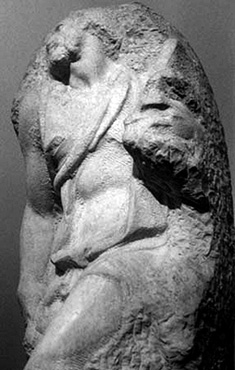
\includegraphics[width=2in]{L1-unfinished.jpg}
    \end{figure}
}

\frame{
\frametitle{V. Vazirani said:  $cont'd$ }

\begin{block}{}
{\it By analogy, we would like to start with a clean, simply stated problem. \\
Most of the algorithm design effort actually goes into \textcolor{red}{\bf understanding the algorithmically relevant combinatorial structure of the problem}. \\
The algorithm exploits this structure in a minimal manner..... \\
with emphasis on stating the structure offered by the problems, and keeping the algorithms minimal.  }
\end{block}

(See extra slides.)
}

%  \frame {
%  \frametitle{A first problem: Regular expression matching problem}
%  Contributed by Yanbing Liu, Security lab at ICT. \\
%  (see extra slides.)
%  }
 
% \frame {
% \frametitle{A first problem: Regular expression matching problem}
% \begin{itemize}
%  \item Key observation: solution=vector;
%  \item Solution space size: $O(\prod_{i=1}^n \mid S_i \mid)$ %$O(prod_{i=1}^n S_i)$
%  \item Brute-force: $O(\prod_{i=1}^n \mid S_i \mid)$ time. 
% \end{itemize}
% 
% \begin{figure}
%         \centering
%         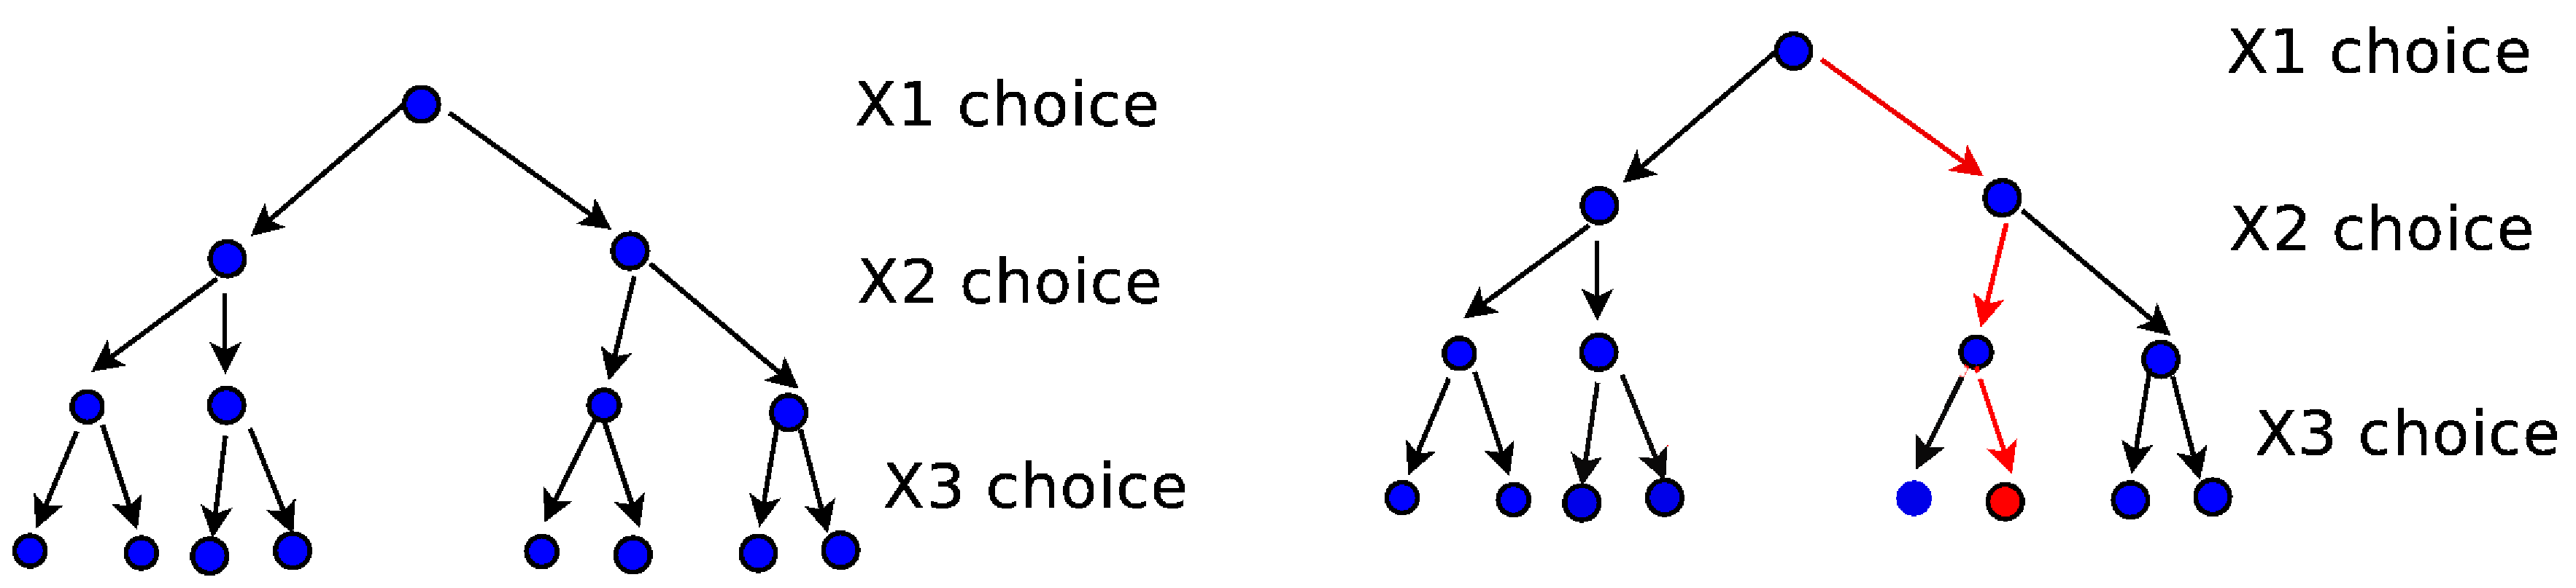
\includegraphics[width=4in]{L1-regularexpressionsearchspace.eps}
% \end{figure}
% }
% 
% 
% \frame {
% \frametitle{A first problem: Regular expression matching problem  $(cont'd)$ }
% \begin{itemize}
%  \item 
% Key observation: solution=vector=path; solution can be decomposed. \\
% \item Key idea: run BFS to check whether the final nodes are reachable; or dynamic programming;
% \item Time-complexity:  $O(4*n)$ \\
% \end{itemize}
% 
% \begin{figure}
%         \centering
%         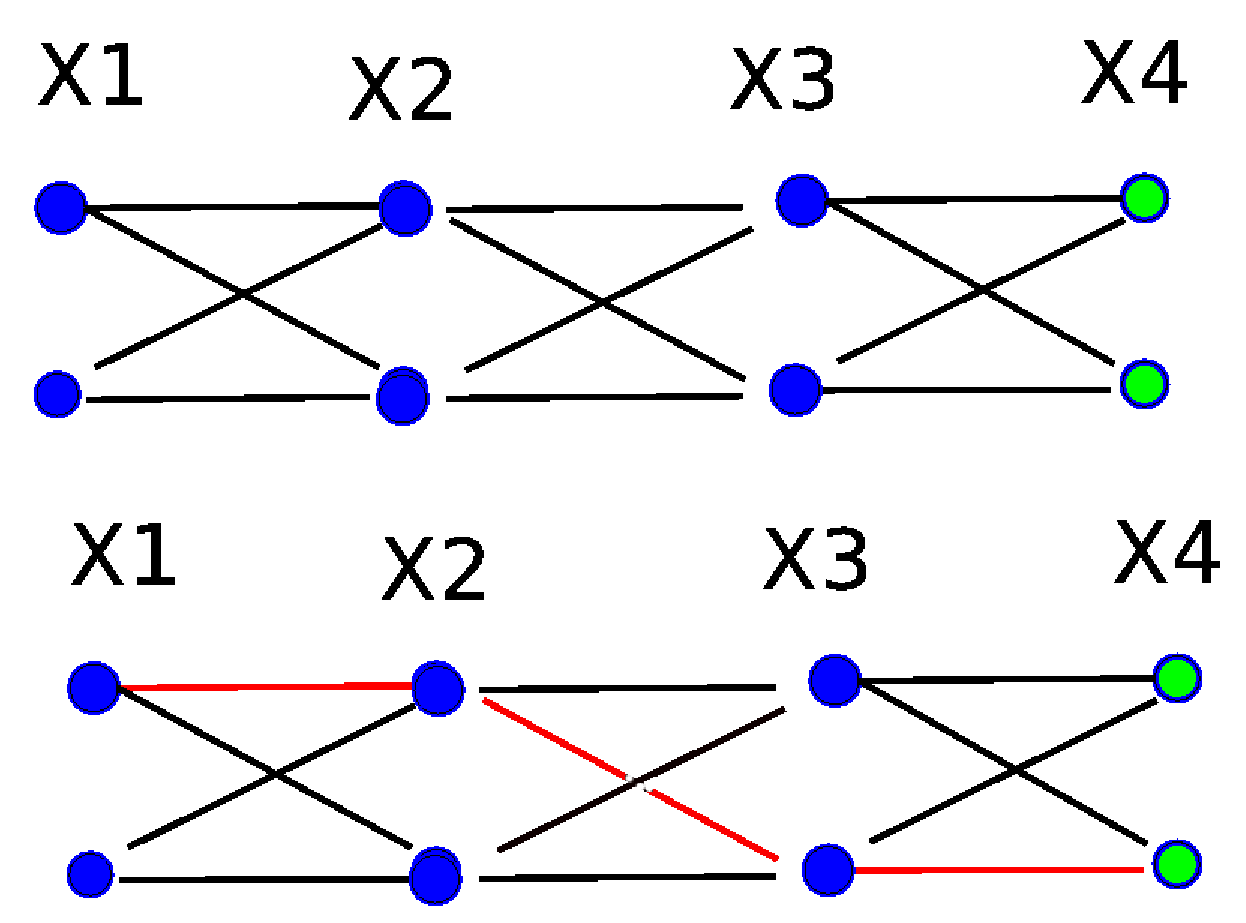
\includegraphics[width=2in]{L1-regularexpressionalgo.eps}
% \end{figure}
% 
%}

\frame{
	\frametitle{Basic algorithmic techniques}
	\begin{itemize}
		\item \textcolor{red}{\bf Divide-and-conquer}: Let's start from the ``smallest" problem first, and investigate whether a large problem can \textcolor{blue}{\bf reduce to smaller  subproblems}.  \\
		
		\item \textcolor{red}{\bf Improvement}: Let's start from  \textcolor{blue}{\bf an initial complete solution}, and try to improve it step by step.  
		\item \textcolor{red}{\bf  ``Intelligent" enumeration}: we enumerate  \textcolor{blue}{\bf all possible complete solutions}, but employ some techniques to prune the search tree. 
	\end{itemize}
}

\frame {
\begin{block}{}
 
 {\bf The first example: calculating the greatest common divisor  ({\bf gcd})}
\end{block}

} 




\frame {
 \frametitle{The first problem: calculating {\bf gcd} }
 \begin{definition}[$\gcd$]
 	The greatest common divisor of two integers $a$ and $b$, when at least one of them is not zero, is the largest positive integer that divides the numbers without a remainder.
 \end{definition}
 \begin{itemize}
\item
	Example: 
 \begin{itemize}
\item The divisors of 54 are: $1, 2, 3, 6, 9, 18, 27, 54$  
\item The divisors of 24 are: $1, 2, 3, 4, 6, 8, 12, 24$ 
\item Thus, $\gcd(54,24) = 6$. 
 \end{itemize}
 \end{itemize}
 }



\frame {
 \frametitle{The first problem: calculating {\bf gcd} }
 
 \begin{block}{}
  {\bf INPUT: } two $n$ bits numbers $a$, and $b$ ($a\geq b$)\\
  {\bf OUTPUT: } $\gcd(a, b)$
  \end{block}

 \begin{itemize}
 	\item Observation: the problem size can be measured by using $n$; 
	\item Let's start from the ``smallest'' instance: $\gcd( 1, 0) = 1$; 
	\item But how to efficiently solve a ``larger'' instance, say $\gcd( 1949,  101)$?
  \end{itemize}
 }
 
\frame {
\frametitle{Euclid's rule} 
 
\begin{figure}
\begin{tikzpicture}[scale=1.1, auto,swap]

    \draw[fill=green!10, rounded corners] (0, 1)  -- (0,0) -- (5, 0) -- (5, 5) -- (0, 5) -- (0, 1); 
            
    \foreach \pos/ \name / \label in {{(2.5,0.5)/gcd01/gcd(1,0)}} 
        \node[smallvertex,fill=red] (\name) at \pos{};
    \foreach \pos/ \name / \label in {{(2.5 + 0.1,0.5)/gcd01/\gcd(1,0)}} 
	   \node[right] at \pos {$\label$}; 

    \foreach \pos/ \name / \label in {{(2.5,4.5)/gcd1949/gcd(1,0)}} 
        \node[smallvertex,fill=blue!20] (\name) at \pos{};
    \foreach \pos/ \name / \label in {{(2.5 + 0.1,4.5)/gcd01/\gcd(1949,101)}} 
	   \node[right] at \pos {$\label$}; 


     
    % Connect vertices with edges and draw weights
%    \foreach \source/ \dest/\weight in {m/w/{}, m'/w'/{} }
%        \path[undirectededge] (\source) -- node[weight] {$\weight$} (\dest);
%       \draw[dashed, ->] (0,0) arc  (120:60:2);

   \node[above] at (2.5, 5.2 ) {Problem instances}; 
   
   
   

       \end{tikzpicture}

\end{figure}
 \begin{itemize}
	\item Observation: a large problem can reduce to a smaller subproblems: 
 	\item $\gcd( 1949, 101) = \gcd( 101, 1949 \mod 101 ) = \gcd( 101, 30)$
 \end{itemize}
}


\frame {
\frametitle{Strategy: reduce to ``smaller" problems} 
 
\begin{figure}
\begin{tikzpicture}[scale=1.1, auto,swap]

   \draw[fill=green!10, rounded corners] (0, 1)  -- (0,0) -- (5, 0) -- (5, 5) -- (0, 5) -- (0, 1); 

        
    \foreach \pos/ \name / \label in {{(2.5,0.5)/gcd01/gcd(1,0)}} 
        \node[smallvertex,fill=red] (\name) at \pos{};
    \foreach \pos/ \name / \label in {{(2.5 + 0.1,0.5)/gcd01/\gcd(1,0)}} 
	   \node[right] at \pos {$\label$}; 

    \foreach \pos/ \name / \label in {{(2.5,4.5)/gcd1949/gcd(1,0)}} 
        \node[smallvertex,fill=blue!20] (\name) at \pos{};
    \foreach \pos/ \name / \label in {{(2.5 + 0.1,4.5)/gcd01/\gcd(1949,101)}} 
	   \node[right] at \pos {$\label$}; 

    \foreach \pos/ \name / \label in {{(2.5,3.5)/gcd101/gcd(1,0)}} 
        \node[smallvertex,fill=blue!20] (\name) at \pos{};
    \foreach \pos/ \name / \label in {{(2.5 + 0.1, 3.5)/gcd01/\gcd(101, 30)}} 
	   \node[right] at \pos {$\label$}; 

    % Connect vertices with edges and draw weights
    \foreach \source/ \dest/\weight in {gcd1949/gcd101/{}}
        \draw[->] (\source) -- node[weight] {$\weight$} (\dest);
%       \draw[dashed, ->] (0,0) arc  (120:60:2);

   \node[above] at (2.5, 5.2 ) {Problem instances}; 
   
       \end{tikzpicture}
\end{figure}

 \begin{itemize}
 	\item $\gcd( 101, 30) = \gcd( 30, 101 \mod 30 ) = \gcd( 30, 11)$
 \end{itemize}
}


\frame {
\frametitle{Strategy: reduce to "smaller" problems} 
 
\begin{figure}
\begin{tikzpicture}[scale=1.1, auto,swap]

   \draw[fill=green!10, rounded corners] (0, 1)  -- (0,0) -- (5, 0) -- (5, 5) -- (0, 5) -- (0, 1); 
        
    \foreach \pos/ \name / \label in {{(2.5,0.5)/gcd01/gcd(1,0)}} 
        \node[smallvertex,fill=red] (\name) at \pos{};
    \foreach \pos/ \name / \label in {{(2.5 + 0.1,0.5)/gcd01/\gcd(1,0)}} 
	   \node[right] at \pos {$\label$}; 

    \foreach \pos/ \name / \label in {{(2.5,4.5)/gcd1949/gcd(1,0)}} 
        \node[smallvertex,fill=blue!20] (\name) at \pos{};
    \foreach \pos/ \name / \label in {{(2.5 + 0.1,4.5)/gcd01/\gcd(1949,101)}} 
	   \node[right] at \pos {$\label$}; 

    \foreach \pos/ \name / \label in {{(2.5,3.5)/gcd101/gcd(1,0)}} 
        \node[smallvertex,fill=blue!20] (\name) at \pos{};
    \foreach \pos/ \name / \label in {{(2.5 + 0.1, 3.5)/gcd01/\gcd(101, 30)}} 
	   \node[right] at \pos {$\label$}; 

    \foreach \pos/ \name / \label in {{(2.5,2.5)/gcd30/gcd(1,0)}} 
        \node[smallvertex,fill=blue!20] (\name) at \pos{};
    \foreach \pos/ \name / \label in {{(2.5 + 0.1, 2.5)/gcd01/\gcd(30, 11)}} 
	   \node[right] at \pos {$\label$}; 


    % Connect vertices with edges and draw weights
    \foreach \source/ \dest/\weight in {gcd1949/gcd101/{},gcd101/gcd30/{}}
        \draw[->] (\source) -- node[weight] {$\weight$} (\dest);
%       \draw[dashed, ->] (0,0) arc  (120:60:2);

   \node[above] at (2.5, 5.2 ) {Problem instances}; 
   
       \end{tikzpicture}
\end{figure}

 \begin{itemize}
 	\item $\gcd( 30, 11) = \gcd( 11, 30 \mod 11 ) = \gcd( 11, 8)$
 \end{itemize}
}

\frame {
\frametitle{Strategy: reduce to "smaller" problems} 
 
\begin{figure}
\begin{tikzpicture}[scale=1.1, auto,swap]

   \draw[fill=green!10, rounded corners] (0, 1)  -- (0,0) -- (5, 0) -- (5, 5) -- (0, 5) -- (0, 1); 
        
    \foreach \pos/ \name / \label in {{(2.5,0.5)/gcd01/gcd(1,0)}} 
        \node[smallvertex,fill=red] (\name) at \pos{};
    \foreach \pos/ \name / \label in {{(2.5 + 0.1,0.5)/gcd01/\gcd(1,0)}} 
	   \node[right] at \pos {$\label$}; 

    \foreach \pos/ \name / \label in {{(2.5,4.5)/gcd1949/gcd(1,0)}} 
        \node[smallvertex,fill=blue!20] (\name) at \pos{};
    \foreach \pos/ \name / \label in {{(2.5 + 0.1,4.5)/gcd01/\gcd(1949,101)}} 
	   \node[right] at \pos {$\label$}; 

    \foreach \pos/ \name / \label in {{(2.5,3.5)/gcd101/gcd(1,0)}} 
        \node[smallvertex,fill=blue!20] (\name) at \pos{};
    \foreach \pos/ \name / \label in {{(2.5 + 0.1, 3.5)/gcd01/\gcd(101, 30)}} 
	   \node[right] at \pos {$\label$}; 

    \foreach \pos/ \name / \label in {{(2.5,2.5)/gcd30/gcd(1,0)}} 
        \node[smallvertex,fill=blue!20] (\name) at \pos{};
    \foreach \pos/ \name / \label in {{(2.5 + 0.1, 2.5)/gcd01/\gcd(30, 11)}} 
	   \node[right] at \pos {$\label$}; 


    % Connect vertices with edges and draw weights
    \foreach \source/ \dest/\weight in {gcd1949/gcd101/{},gcd101/gcd30/{}}
        \draw[->] (\source) -- node[weight] {$\weight$} (\dest);
%       \draw[dashed, ->] (0,0) arc  (120:60:2);

    \foreach \source/ \dest/\weight in {gcd30/gcd01/{}}
        \draw[dashed, ->] (\source) -- node[weight] {$\weight$} (\dest);
%       \draw[dashed, ->] (0,0) arc  (120:60:2);

   \node[above] at (2.5, 5.2 ) {Problem instances}; 
       \end{tikzpicture}
\end{figure}

 \begin{itemize}
 	\item $\gcd( 30, 11) =  \gcd( 11, 8) = \gcd(8, 3) = \gcd( 3, 2) = \gcd( 2, 1) = \gcd( 1, 0) = 1  $
 \end{itemize}
}

\frame {
\frametitle{Sub-instance relationship graph} 
 
\begin{figure}
\begin{tikzpicture}[scale=1.1, auto,swap]

   \draw[fill=green!10, rounded corners] (0, 1)  -- (0,0) -- (5, 0) -- (5, 5) -- (0, 5) -- (0, 1); 
        
    \foreach \pos/ \name / \label in {{(2.5,0.5)/gcd01/gcd(1,0)}} 
        \node[smallvertex,fill=red] (\name) at \pos{};
    \foreach \pos/ \name / \label in {{(2.5 + 0.1,0.5)/gcd01/\gcd(1,0)}} 
	   \node[right] at \pos {$\label$}; 

    \foreach \pos/ \name / \label in {{(2.5,4.5)/gcd1949/gcd(1,0)}} 
        \node[smallvertex,fill=blue!20] (\name) at \pos{};
    \foreach \pos/ \name / \label in {{(2.5 + 0.1,4.5)/gcd01/\gcd(1949,101)}} 
	   \node[right] at \pos {$\label$}; 

    \foreach \pos/ \name / \label in {{(2.5,3.5)/gcd101/gcd(1,0)}} 
        \node[smallvertex,fill=blue!20] (\name) at \pos{};
    \foreach \pos/ \name / \label in {{(2.5 + 0.1, 3.5)/gcd01/\gcd(101, 30)}} 
	   \node[right] at \pos {$\label$}; 

    \foreach \pos/ \name / \label in {{(2.5,2.5)/gcd30/gcd(1,0)}} 
        \node[smallvertex,fill=blue!20] (\name) at \pos{};
    \foreach \pos/ \name / \label in {{(2.5 + 0.1, 2.5)/gcd01/\gcd(30, 11)}} 
	   \node[right] at \pos {$\label$}; 


    % Connect vertices with edges and draw weights
    \foreach \source/ \dest/\weight in {gcd1949/gcd101/{},gcd101/gcd30/{}}
        \draw[->] (\source) -- node[weight] {$\weight$} (\dest);
%       \draw[dashed, ->] (0,0) arc  (120:60:2);

    \foreach \source/ \dest/\weight in {gcd30/gcd01/{}}
        \draw[dashed, ->] (\source) -- node[weight] {$\weight$} (\dest);
%       \draw[dashed, ->] (0,0) arc  (120:60:2);

   \node[above] at (2.5, 5.2 ) {Problem instances}; 
       \end{tikzpicture}
\end{figure}

 \begin{itemize}
 	\item Node: subproblems 
	\item Edge: reduction relationship 
 \end{itemize}
}

\frame {
\frametitle{Euclid algorithm } 


\begin{algorithmic}[1]
\STATE{ {\bf function} Euclid}{($a,b$)}
%\STATE { /* $a$ and $b$ are integers, and $a \geq b \geq 0$ */ }  
\IF{ $ b = 0 $ }  
	\RETURN $a$; 
\ENDIF
\RETURN{ Euclid( $b$, $a \mod b$) }; 
\end{algorithmic}
} 

\frame {
\frametitle{Time complexity analysis } 

\begin{Theorem}
Suppose $a$ is a $n$-digit integer. Euclid($a$, $b$) ends in $O(n^3)$ time. 
\end{Theorem}
\begin{Proof}
	\begin{itemize}
		\item There are at most $2n$ recursive calling. 
			\begin{itemize}
				\item Note that $ a \mod b < \frac{a}{2}$. 
				\item After two rounds of recursive calling, both $a$ and $b$ shrink at least a half size. 
			\end{itemize}
		\item At each recursive calling, the $\mod$ operation costs $O(n^2)$ time. 
	\end{itemize}
\end{Proof}

} 

\frame{
\begin{block}{}
{\bf The second example: travelling salesman problem (TSP)}
\end{block}

}



\frame{
	\frametitle{TSP: a concrete example } 
	
	\begin{figure}
	\begin{minipage}{1in}
        	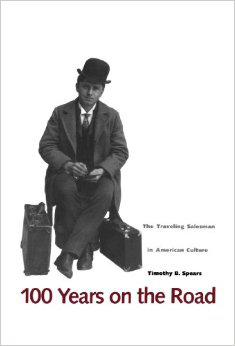
\includegraphics[width=\textwidth]{TSP-100years.png}
	\end{minipage}
	\begin{minipage}{1.5in}
        	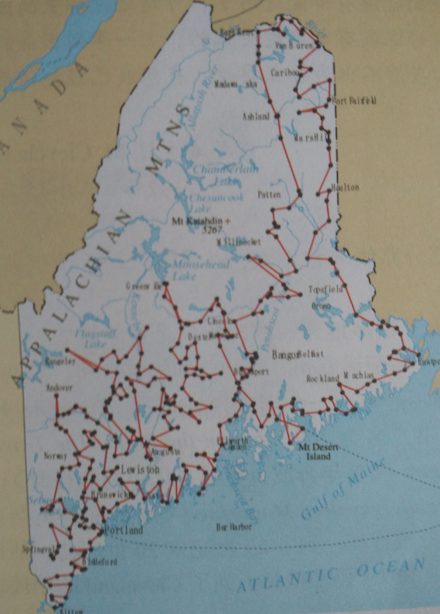
\includegraphics[width=\textwidth]{TSP-350.png}
	\end{minipage}
    \end{figure}
\begin{itemize}
	\item In 1925, H. M. Cleveland, a salesman of the Page seed company, traveled 350 cities to gather order form. 
	\item Of course, the shorter the total distance, the better. 
\end{itemize}
}


\frame{
	\frametitle{How did they do? Pin and wire! } 
	
	\begin{figure}
	\begin{minipage}{2in}
        	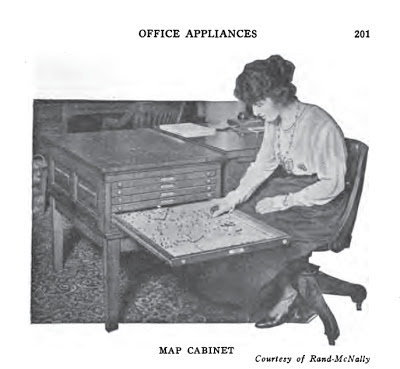
\includegraphics[width=\textwidth]{TSP-Secretary.jpg}
	\end{minipage}
	\begin{minipage}{1.5in}
        	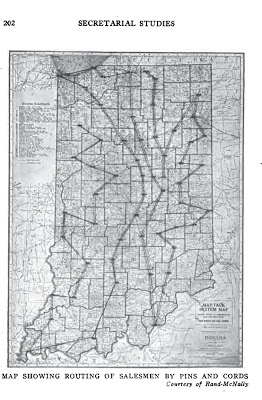
\includegraphics[width=\textwidth]{TSP-Secretary2.jpg}
	\end{minipage}
    \end{figure}
\begin{itemize}
	\item Two pictures excerpted from {\it Secretarial Studies}, 1922. 
\end{itemize}
}



\frame{
	\frametitle{ {\sc Travelling Salesman Problem}  } 

	\begin{block}{}
		{\bf INPUT:  } a list of $n$ cities $V=\{1, 2, ..., n\}$,  and a distance matrix $D$, where $d_{ij}$ $(1\leq i, j \leq n)$ denotes the distance between city $i$ and $j$ \\ 
		{\bf OUTPUT: }  the shortest tour that visits each city exactly once and returns to the origin city 
	\end{block} 	
	
\begin{figure}
	\begin{tikzpicture}[scale=1, auto,swap]

    \foreach \pos/ \name in {{(0,0)/1},{(0,2)/2}, {(2,2)/3}, {(2,0)/4}} 
        \node[smallvertex,fill=blue!20] (\name) at \pos{$\name$};

     
    % Connect vertices with edges and draw weights
    \foreach \source/ \dest/\weight in {2/1/{1},   1/4/{3}, 3/2/{5}, 4/3/{3}}
        \path[undirectededge] (\source) -- node[weight] {$\weight$} (\dest);
    \foreach \source/ \dest/\weight in  {3/1/{8}, 4/2/{7}}
        \path[undirectededge] (\source) -- node[weight] {$\weight$} (\dest);
        
	\end{tikzpicture}
\end{figure}
$\#$Tours:  $6$
\begin{itemize}
	\item Tour 1: $1\rightarrow 2 \rightarrow 3 \rightarrow 4 \rightarrow 1$ (distance: 12)
	\item Tour 2: $1\rightarrow 2 \rightarrow 4 \rightarrow 3 \rightarrow 1$ (distance: 21)
	\item Tour 3: $1\rightarrow 3 \rightarrow 2 \rightarrow 4 \rightarrow 1$ (distance: 23)
	\item ....
\end{itemize}

}


\frame{
\begin{block}{}
{\bf Trial 1: divide and conquer}
\end{block}
}

\frame{
	\frametitle{Consider a tightly  related problem }

\begin{figure}
	\begin{tikzpicture}[scale=1, auto,swap]

    \foreach \pos/ \name in {{(0,0)/1},{(0,1.5)/2}, {(1.5,1.5)/3}, {(1.5,0)/4}} 
        \node[smallvertex,fill=blue!20] (\name) at \pos{$\name$};

     
    % Connect vertices with edges and draw weights
    \foreach \source/ \dest/\weight in {2/1/{1},   1/4/{3}, 3/2/{5}, 4/3/{3}}
        \path[undirectededge] (\source) -- node[weight] {$\weight$} (\dest);
    \foreach \source/ \dest/\weight in  {3/1/{8}, 4/2/{7}}
        \path[undirectededge] (\source) -- node[weight] {$\weight$} (\dest);
        
	\end{tikzpicture}
\end{figure}


	\begin{definition}{}
		$D(S, e) = $ the minimum distance, starting from city $1$, visiting all cities in $S$ once and exactly once, and finishing at city $e$. 
	\end{definition} 
	
	\begin{itemize}
%		\item Note the solution is a tour of the $n$ cities. 
		\item There are 3 cases of the city from which we return to $1$. 
		\item Thus, the shortest tour can be calculated as: \\ $\min\{ d_{2,1} + D( \{ 3, 4\}, 2)$, \\$ d_{3,1} + D( \{2, 4\}, 3 )$, \\ $d_{4,1} + D( \{ 2, 3\}, 4 )   \}$
	\end{itemize}

}



\frame{
	\frametitle{Consider the smallest problem }


	\begin{itemize}
		\item It is trivial to calculate $D( S, e)$ when $S$ consists of only 1 city. 
\begin{figure}
	\begin{tikzpicture}[scale=1, auto,swap]

    \foreach \pos/ \name in {{(0,0)/1},{(0,1.5)/2}, {(2,1.5)/3}} 
        \node[smallvertex,fill=blue!20] (\name) at \pos{$\name$};

    % Connect vertices with edges and draw weights
    \foreach \source/ \dest/\weight in {2/1/{1},   3/2/{5}}
        \path[undirectededge] (\source) -- node[weight] {$\weight$} (\dest);
    \foreach \source/ \dest/\weight in  {3/1/{8}}
        \path[undirectededge] (\source) -- node[weight] {$\weight$} (\dest);

    \foreach \source/ \dest/\weight in {2/1/{},   3/2/{}}
        \path[undirectededge, red] (\source) -- node[weight] {$\weight$} (\dest);
        

    \foreach \pos/ \name in {{(3,0)/1},{(3,1.5)/2}, {(5,1.5)/3}} 
        \node[smallvertex,fill=blue!20] (\name) at \pos{$\name$};

    % Connect vertices with edges and draw weights
    \foreach \source/ \dest/\weight in {2/1/{1},   3/2/{5}}
        \path[undirectededge] (\source) -- node[weight] {$\weight$} (\dest);
    \foreach \source/ \dest/\weight in  {3/1/{8}}
        \path[undirectededge] (\source) -- node[weight] {$\weight$} (\dest);

    \foreach \source/ \dest/\weight in {2/3/{},   3/1/{}}
        \path[undirectededge, red] (\source) -- node[weight] {$\weight$} (\dest);
        
        
	\end{tikzpicture}


\end{figure}


		\item $D( \{ 2\}, 3) = d_{12} + d_{23}$ $\qquad$ $D( \{  3\}, 2) = d_{13} + d_{32}$
		\item But how to solve a larger problem, say $D(\{2, 3\}, 4)$?
	\end{itemize}
}

\frame{
	\frametitle{Sub-instance relationship graph}
	\begin{figure}
\begin{tikzpicture}[scale=1.1, auto,swap]

   \draw[fill=green!10, rounded corners] (0, 1)  -- (0,0) -- (5, 0) -- (5, 5) -- (0, 5) -- (0, 1); 
        
    \foreach \pos/ \name / \label in {{(2.5,3.5)/D1234/}} 
        \node[smallvertex,fill=blue!20] (\name) at \pos{};
    \foreach \pos/ \name / \label in {{(2.5 + 0.1, 3.5)/D1234/D(\{2,3\}, 4)}} 
	   \node[right] at \pos {\small $\label$}; 

    \foreach \pos/ \name / \label in {{(2,1.5)/D1232/}} 
        \node[smallvertex,fill=red] (\name) at \pos{};
    \foreach \pos/ \name / \label in {{(2 - 0.1, 1.5)/D1232/D(\{3\}, 2) }} 
	   \node[left] at \pos {\small $\label$}; 

    \foreach \pos/ \name / \label in {{(3,1.5)/D1233/}} 
        \node[smallvertex,fill=red] (\name) at \pos{};
    \foreach \pos/ \name / \label in {{(3 + 0.1, 1.5)/D1233/D(\{2\}, 3) }} 
	   \node[right] at \pos {\small $\label$}; 


   \node[above] at (2.5, 5.2 ) {Problem instances}; 
       \end{tikzpicture}
\end{figure}

}



\frame{
	\frametitle{Divide a larger problem into smaller problems }

\begin{figure}
	\begin{tikzpicture}[scale=1, auto,swap]

    \foreach \pos/ \name in {{(0,0)/1},{(0,1.5)/2}, {(1.5,1.5)/3}, {(1.5,0)/4}} 
        \node[smallvertex,fill=blue!20] (\name) at \pos{$\name$};

     
    % Connect vertices with edges and draw weights
    \foreach \source/ \dest/\weight in {2/1/{1},   1/4/{3}, 3/2/{5}, 4/3/{3}}
        \path[undirectededge] (\source) -- node[weight] {$\weight$} (\dest);
    \foreach \source/ \dest/\weight in  {3/1/{8}, 4/2/{7}}
        \path[undirectededge] (\source) -- node[weight] {$\weight$} (\dest);

%red 	
    \foreach \source/ \dest/\weight in  {1/2/{}, 2/3/{}, 4/3/{}}
        \path[undirectededge,red] (\source) -- node[weight] {$\weight$} (\dest);




    \foreach \pos/ \name in {{(3,0)/1},{(3,1.5)/2}, {(4.5,1.5)/3}, {(4.5,0)/4}} 
        \node[smallvertex,fill=blue!20] (\name) at \pos{$\name$};

     
    % Connect vertices with edges and draw weights
    \foreach \source/ \dest/\weight in {2/1/{1},   1/4/{3}, 3/2/{5}, 4/3/{3}}
        \path[undirectededge] (\source) -- node[weight] {$\weight$} (\dest);
    \foreach \source/ \dest/\weight in  {3/1/{8}, 4/2/{7}}
        \path[undirectededge] (\source) -- node[weight] {$\weight$} (\dest);

%red 	
    \foreach \source/ \dest/\weight in  {1/3/{}, 2/3/{}, 4/2/{}}
        \path[undirectededge,red] (\source) -- node[weight] {$\weight$} (\dest);

        
	\end{tikzpicture}
\end{figure}

	\begin{itemize}
		\item $D( \{2, 3\}, 4) = \min\{ d_{34} + D( \{2\}, 3), d_{24} + D( \{ 3\}, 2)  \} $
	\end{itemize}
}

\frame{
	\frametitle{Reduce to smaller problems }
	\begin{figure}
\begin{tikzpicture}[scale=1.1, auto,swap]

   \draw[fill=green!10, rounded corners] (0, 1)  -- (0,0) -- (5, 0) -- (5, 5) -- (0, 5) -- (0, 1); 
        
    \foreach \pos/ \name / \label in {{(2.5,3.5)/D1234/}} 
        \node[smallvertex,fill=blue!20] (\name) at \pos{};
    \foreach \pos/ \name / \label in {{(2.5 + 0.1, 3.5)/D1234/D(\{2,3,4\}, 4)}} 
	   \node[right] at \pos {\small $\label$}; 

    \foreach \pos/ \name / \label in {{(2,1.5)/D1232/}} 
        \node[smallvertex,fill=red] (\name) at \pos{};
    \foreach \pos/ \name / \label in {{(2 - 0.1, 1.5)/D1232/D(\{2,3\}, 2) }} 
	   \node[left] at \pos {\small $\label$}; 

    \foreach \pos/ \name / \label in {{(3,1.5)/D1233/}} 
        \node[smallvertex,fill=red] (\name) at \pos{};
    \foreach \pos/ \name / \label in {{(3 + 0.1, 1.5)/D1233/D(\{2,3\}, 3) }} 
	   \node[right] at \pos {\small $\label$}; 

    % Connect vertices with edges and draw weights
    \foreach \source/ \dest/\weight in {D1234/D1232/{},D1234/D1233/{}}
        \draw[->] (\source) -- node[weight] {$\weight$} (\dest);
%       \draw[dashed, ->] (0,0) arc  (120:60:2);

   \node[above] at (2.5, 5.2 ) {Problem instances}; 
       \end{tikzpicture}
\end{figure}

}

\frame{
	\frametitle{ Held-Karp algorithm [1962]} 

\begin{algorithmic}[1]
\STATE{ {\bf function} $TSP(V, D)$ }
\RETURN{$\min_{e \in V, e \neq 1}D( V - \{e\}, e) + d_{e1}$}; 
\end{algorithmic}
\quad \\
\quad \\
\begin{algorithmic}[1]
\STATE{ {\bf function} $D(S, e)$ }
\IF{ $ S = \{v\}$ }
	\STATE $D(S, e) = d_{1v} + d_{ve}$; 
	\RETURN{$D( S, e)$}; 
\ENDIF
\RETURN{$\min_{i \in S, i \neq e}D( S - \{i\}, i) + d_{ei}$}; 
\end{algorithmic}


\begin{itemize}
	\item Time complexity: $O( 2^n n^2)$. 
\end{itemize}
	
} 
	


\frame{
\begin{block}{}
{\bf Trial 2: Improvement strategy  }
\end{block}
}

\frame{
	\frametitle{Solution space  }

\begin{figure}
        \centering
        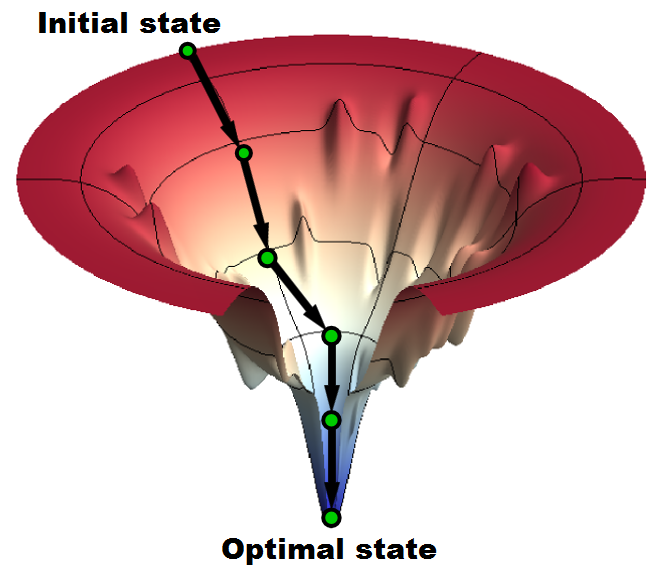
\includegraphics[width=2in]{Landscape.png}
%	\caption{\tiny Muhammad ibn Musa al-Khwarizmi (C. 780---850), a Persian scholar, formerly Latinized as Algoritmi}
\end{figure}
\begin{itemize}
	\item Node: a complete solution. Each node is associated with an objective function value. 
	\item Edge: if two nodes are neighboors, an edge is added to connect them. Here "neighbours" refers to two nodes with small difference. 
	\item Improvement strategy:  start from an initial solution, and try to improve it step by step. 
\end{itemize}

    
} 

\frame{
	\frametitle{ {\sc Improvement} strategy }

\begin{figure}
	\begin{tikzpicture}[scale=1, auto,swap]

    \foreach \pos/ \name in {{(0,0)/1},{(0,2)/2}, {(2,2)/3}, {(2,0)/4}} 
        \node[smallvertex,fill=blue!20] (\name) at \pos{$\name$};

     
    % Connect vertices with edges and draw weights
    \foreach \source/ \dest/\weight in {2/1/{1},   1/4/{3}, 3/2/{5}, 4/3/{3}}
        \path[undirectededge] (\source) -- node[weight] {$\weight$} (\dest);
    \foreach \source/ \dest/\weight in  {3/1/{8}, 4/2/{7}}
        \path[undirectededge] (\source) -- node[weight] {$\weight$} (\dest);
        
	\end{tikzpicture}
\end{figure}

	\begin{itemize}
		\item Note that a \textcolor{red}{\bf complete solution} can be expressed as a  permutations of the $n$ cities; 
		\item Let's start from \textcolor{red}{\bf an initial  complete solution}, and try to improve it;
	\end{itemize} 
	
	 
}


\frame{
	\frametitle{ {\sc Improvement} strategy }

%\begin{figure}
%	\begin{tikzpicture}[scale=0.8, auto,swap]
%
%    \foreach \pos/ \name in {{(0,0)/1},{(0,2)/2}, {(2,2)/3}, {(2,0)/4}} 
%        \node[smallvertex,fill=blue!20] (\name) at \pos{$\name$};
%
%     
%    % Connect vertices with edges and draw weights
%    \foreach \source/ \dest/\weight in {2/1/{1},   1/4/{3}, 3/2/{5}, 4/3/{3}}
%        \path[undirectededge] (\source) -- node[weight] {$\weight$} (\dest);
%    \foreach \source/ \dest/\weight in  {3/1/{8}, 4/2/{7}}
%        \path[undirectededge] (\source) -- node[weight] {$\weight$} (\dest);
%        
%	\end{tikzpicture}
%\end{figure}

	
	\begin{algorithmic}[1]
\STATE Let $s$ be an initial tour; 
\WHILE{ {\tt TRUE} }
	\STATE select a new tour $s'$ from the \textcolor{red}{\bf neighbourhood} of $s$; 
	\IF{ $s'$ is shorter than $s$ }  
		\STATE $s = s'$; 
	\ENDIF
	\IF{ stopping($s$)}
		\RETURN{ $s$}; 
	\ENDIF
\ENDWHILE
\end{algorithmic}
Here, \textcolor{red}{\bf neighbourhood} is introduced to describe how to change an existing tour into a new one;  
	 
}

\frame{
	\frametitle{But how to define neighbourhood of a tour? } 
	\begin{itemize}
		\item 2-opt strategy: if $s'$ and $s$ differ at only two edges (Note: 1-opt is impossible)
	\end{itemize}

\begin{figure}
	\begin{tikzpicture}[scale=1, auto,swap]

    \foreach \pos/ \name in {{(0,0)/1},{(0,2)/2}, {(2,2)/3}, {(2,0)/4}} 
        \node[smallvertex,fill=blue!20] (\name) at \pos{$\name$};
    
    % Connect vertices with edges and draw weights
    \foreach \source/ \dest/\weight in {2/1/{1},   3/4/{3} }
        \path[undirectededge] (\source) -- node[weight] { } (\dest);
    \foreach \source/ \dest/\weight in  {3/1/{8}, 4/2/{7}}
        \path[undirectededge, red] (\source) -- node[weight] { } (\dest);
 
 	\node[] at (1, -0.5) {$s$}; 

 	\node[] at (5, -0.5) {$s'$}; 
   
   \draw[->, blue, line width=2pt] (2.6, 1) -- (3.4, 1);
 

    \foreach \pos/ \name in {{(4,0)/1},{(4,2)/2}, {(6,2)/3}, {(6,0)/4}} 
        \node[smallvertex,fill=blue!20] (\name) at \pos{$\name$};
    
    % Connect vertices with edges and draw weights
    \foreach \source/ \dest/\weight in {2/1/{1},   3/4/{3} }
        \path[undirectededge] (\source) -- node[weight] { } (\dest);
    \foreach \source/ \dest/\weight in  {4/1/{8}, 3/2/{7}}
        \path[undirectededge, red] (\source) -- node[weight] { } (\dest);
        
 
        
	\end{tikzpicture}
\end{figure}
		
}


\frame{
	\frametitle{An example} 
		
\begin{figure}
	\begin{tikzpicture}[scale=1, auto,swap]

    \foreach \pos/ \name in {{(-2,0)/a},{(2,0)/b}, {(-1,1.6)/e}, {(1,1.6)/c}, {(0,3.2)/d}} 
        \node[smallvertex,fill=blue!20] (\name) at \pos{$\name$};
     
    % Connect vertices with edges and draw weights
     %   \foreach \source/ \dest/\weight in {a/b/{3},   c/a/{4}, e/a/{7}, a/d/{2}, b/c/{4}, b/d/{6}, e/b/{3}, c/d/{5}, c/e/{8}, d/e/{6}}
    \foreach \source/ \dest/\weight in {a/b/{3},   a/c/{4}, e/a/{7}, b/c/{4}, e/b/{3}, c/d/{5}, c/e/{8}, d/e/{6}}
        \path[undirectededge] (\source) -- node[weight] {\small $\weight$} (\dest);
         
    \draw[thick] (a)   to [out=140, in=180] node[above] {2} (d);   
        \draw[thick] (b)   to [out=40, in=0] node[above] {6} (d);   
\end{tikzpicture}
\end{figure}


}

\frame{
	\frametitle{Initial tour $s$} 

\begin{figure}
	\begin{tikzpicture}[scale=1, auto,swap]

    \foreach \pos/ \name in {{(-2,0)/a},{(2,0)/b}, {(-1,1.6)/e}, {(1,1.6)/c}, {(0,3.2)/d}} 
        \node[smallvertex,fill=blue!20] (\name) at \pos{$\name$};
     
    % Connect vertices with edges and draw weights
     %   \foreach \source/ \dest/\weight in {a/b/{3},   c/a/{4}, e/a/{7}, a/d/{2}, b/c/{4}, b/d/{6}, e/b/{3}, c/d/{5}, c/e/{8}, d/e/{6}}
    \foreach \source/ \dest/\weight in {a/b/{3},   a/c/{4}, e/a/{7}, b/c/{4}, e/b/{3}, c/d/{5}, c/e/{8}, d/e/{6}}
        \path[undirectededge] (\source) -- node[weight] {\small $\weight$} (\dest);
         
    \draw[thick] (a)   to [out=140, in=180] node[above] {2} (d);   
        \draw[thick] (b)   to [out=40, in=0] node[above] {6} (d);   
        
       \foreach \source/ \dest/\weight in {a/b/,   b/c/,  c/d/, d/e/, e/a/}
        \path[undirectededge, blue] (\source) -- node[weight] {$\weight$} (\dest);


\end{tikzpicture}
\end{figure}


Initial complete solution $s$:  $a \rightarrow b\rightarrow c\rightarrow  d\rightarrow  e\rightarrow a $  (distance: 25)
}


\frame{
	\frametitle{A 2-opt operation: $s \Rightarrow s'$ } 
	
\begin{figure}
	\begin{tikzpicture}[scale=1, auto,swap]

    \foreach \pos/ \name in {{(-2,0)/a},{(2,0)/b}, {(-1,1.6)/e}, {(1,1.6)/c}, {(0,3.2)/d}} 
        \node[smallvertex,fill=blue!20] (\name) at \pos{$\name$};
     
    % Connect vertices with edges and draw weights
     %   \foreach \source/ \dest/\weight in {a/b/{3},   c/a/{4}, e/a/{7}, a/d/{2}, b/c/{4}, b/d/{6}, e/b/{3}, c/d/{5}, c/e/{8}, d/e/{6}}
    \foreach \source/ \dest/\weight in {a/b/{3},   a/c/{4}, e/a/{7}, b/c/{4}, e/b/{3}, c/d/{5}, c/e/{8}, d/e/{6}}
        \path[undirectededge] (\source) -- node[weight] {\small $\weight$} (\dest);
         
    \draw[thick] (a)   to [out=140, in=180] node[above] {2} (d);   
        \draw[thick] (b)   to [out=40, in=0] node[above] {6} (d);   
        
    \foreach \source/ \dest/\weight in {a/b/,   b/c/,  c/d/, d/e/, e/a/}
        \path[undirectededge, blue] (\source) -- node[weight] {$\weight$} (\dest);

    \foreach \source/ \dest/\weight in { e/c/}
        \path[undirectededge, red] (\source) -- node[weight] {$\weight$} (\dest);
 
         
    \foreach \source/ \dest/\weight in {   d/c/,   e/a/}
        \path[undirectededge, yellow] (\source) -- node[weight] {$\weight$} (\dest);


   \draw[thick, red] (a)   to [out=140, in=180] (d);   
 
 \draw[->, line width=3pt, green] (2.7, 1.5) -- (3.3, 1.5); 
 
 \def\dx{6};
 
     \foreach \pos/ \name in {{(-2 + \dx ,0)/a},{(2+ \dx ,0)/b}, {(-1+ \dx ,1.6)/e}, {(1+ \dx ,1.6)/c}, {(0+ \dx ,3.2)/d}} 
        \node[smallvertex,fill=blue!20] (\name) at \pos{$\name$};
     
    % Connect vertices with edges and draw weights
     %   \foreach \source/ \dest/\weight in {a/b/{3},   c/a/{4}, e/a/{7}, a/d/{2}, b/c/{4}, b/d/{6}, e/b/{3}, c/d/{5}, c/e/{8}, d/e/{6}}
    \foreach \source/ \dest/\weight in {a/b/{3},   a/c/{4}, e/a/{7}, b/c/{4}, e/b/{3}, c/d/{5}, c/e/{8}, d/e/{6}}
        \path[undirectededge] (\source) -- node[weight] {\small $\weight$} (\dest);
         
    \draw[thick] (a)   to [out=140, in=180] node[above] {2} (d);   
        \draw[thick] (b)   to [out=40, in=0] node[above] {6} (d);   

    \foreach \source/ \dest/\weight in {a/b/,   b/c/,   d/e/, e/c/}
        \path[undirectededge, blue] (\source) -- node[weight] {$\weight$} (\dest);

    \draw[thick,blue] (a)   to [out=140, in=180] node[above] {2} (d);   


\end{tikzpicture}
\end{figure}
Initial  solution $s$:  $a \rightarrow b\rightarrow c\rightarrow  d\rightarrow  e\rightarrow a $  (distance: 25)

Improve from $s$ to $s'$: $a \rightarrow b\rightarrow c\rightarrow  e\rightarrow  d\rightarrow a $  (distance: 23)

}



\frame{
	\frametitle{One more 2-opt operation: $s' \Rightarrow s''$ } 
	
\begin{figure}
	\begin{tikzpicture}[scale=1, auto,swap]

\def\dx{0};
 
     \foreach \pos/ \name in {{(-2 + \dx ,0)/a},{(2+ \dx ,0)/b}, {(-1+ \dx ,1.6)/e}, {(1+ \dx ,1.6)/c}, {(0+ \dx ,3.2)/d}} 
        \node[smallvertex,fill=blue!20] (\name) at \pos{$\name$};
     
    % Connect vertices with edges and draw weights
     %   \foreach \source/ \dest/\weight in {a/b/{3},   c/a/{4}, e/a/{7}, a/d/{2}, b/c/{4}, b/d/{6}, e/b/{3}, c/d/{5}, c/e/{8}, d/e/{6}}
    \foreach \source/ \dest/\weight in {a/b/{3},   a/c/{4}, e/a/{7}, b/c/{4}, e/b/{3}, c/d/{5}, c/e/{8}, d/e/{6}}
        \path[undirectededge] (\source) -- node[weight] {\small $\weight$} (\dest);
         
    \draw[thick] (a)   to [out=140, in=180] node[above] {2} (d);   
        \draw[thick] (b)   to [out=40, in=0] node[above] {6} (d);   

    \foreach \source/ \dest/\weight in {a/b/,   b/c/,   d/e/, e/c/}
        \path[undirectededge, blue] (\source) -- node[weight] {$\weight$} (\dest);

    \foreach \source/ \dest/\weight in {a/b/,   e/c/}
        \path[undirectededge, yellow] (\source) -- node[weight] {$\weight$} (\dest);


  \draw[thick,blue] (a)   to [out=140, in=180] node[above] {2} (d);   


    \foreach \source/ \dest/\weight in {b/e/,  a/c/}
        \path[undirectededge, red] (\source) -- node[weight] {$\weight$} (\dest);


 \draw[->, line width=3pt, green] (2.7, 1.5) -- (3.3, 1.5); 
 
 \def\dx{6};
 
     \foreach \pos/ \name in {{(-2 + \dx ,0)/a},{(2+ \dx ,0)/b}, {(-1+ \dx ,1.6)/e}, {(1+ \dx ,1.6)/c}, {(0+ \dx ,3.2)/d}} 
        \node[smallvertex,fill=blue!20] (\name) at \pos{$\name$};
     
    % Connect vertices with edges and draw weights
     %   \foreach \source/ \dest/\weight in {a/b/{3},   c/a/{4}, e/a/{7}, a/d/{2}, b/c/{4}, b/d/{6}, e/b/{3}, c/d/{5}, c/e/{8}, d/e/{6}}
    \foreach \source/ \dest/\weight in {a/b/{3},   a/c/{4}, e/a/{7}, b/c/{4}, e/b/{3}, c/d/{5}, c/e/{8}, d/e/{6}}
        \path[undirectededge] (\source) -- node[weight] {\small $\weight$} (\dest);
         
    \draw[thick] (a)   to [out=140, in=180] node[above] {2} (d);   
        \draw[thick] (b)   to [out=40, in=0] node[above] {6} (d);   

    \foreach \source/ \dest/\weight in {b/e/,   b/c/,   d/e/, a/c/}
        \path[undirectededge, blue] (\source) -- node[weight] {$\weight$} (\dest);

   \draw[thick, blue] (a)   to [out=140, in=180] node[above] {2} (d);   

 \end{tikzpicture}
\end{figure}
\begin{itemize}

\item A complete solution $s'$: $a \rightarrow b\rightarrow c\rightarrow  e\rightarrow  d\rightarrow a $  (distance: 23)

\item Improve from $s'$ to $s''$:  $a \rightarrow c\rightarrow b\rightarrow  e\rightarrow  d\rightarrow a $  (distance: 19)

\item Done! No 2-OPT can be found to improve further. 

\end{itemize}

}

\frame{
\begin{block}{}
{\bf Trial 3: ``Intelligent" enumeration strategy }
\end{block}
}


\frame{
	\frametitle{ Solution form }
	%{\sc Backtracking}: enumerate all possible complete solutions }

	\begin{itemize}
		\item Note that a complete solution can be expressed as a sequence of $n-1$ edges. Given a certain order of the $m$ edges, a complete solution can be represented as $X = [x_{1}, x_{2}, ..., x_{m}]$, $x_{i}=0/1$. If the edge $i$ was used, we set $x_i = 1$, and otherwise $x_i=0$. 
		\item For example, the tour $a \rightarrow b\rightarrow c\rightarrow  d\rightarrow  e\rightarrow a $ can be represented as $X=[1, 0, 0, 1, 1, 0, 0, 1, 0, 1]$ under the order $e_1=<a, b>, e_2=<a, c>, e_3 = <a, d>, e_4=<b, c>, e_5=<b, d>, e_6 = <b, e>, e_7=<c, d>, e_8=<c, e>, e_9=<d,e>$.  
	\end{itemize} 

\begin{figure}
	\begin{tikzpicture}[scale=0.9, auto,swap]

    \foreach \pos/ \name in {{(-2,0)/a},{(2,0)/b}, {(-1,1.6)/e}, {(1,1.6)/c}, {(0,3.2)/d}} 
        \node[smallvertex,fill=blue!20] (\name) at \pos{$\name$};
     
    % Connect vertices with edges and draw weights
     %   \foreach \source/ \dest/\weight in {a/b/{3},   c/a/{4}, e/a/{7}, a/d/{2}, b/c/{4}, b/d/{6}, e/b/{3}, c/d/{5}, c/e/{8}, d/e/{6}}
    \foreach \source/ \dest/\weight in {a/b/{3},   a/c/{4}, e/a/{7}, b/c/{4}, e/b/{3}, c/d/{5}, c/e/{8}, d/e/{6}}
        \path[undirectededge] (\source) -- node[weight] {\small $\weight$} (\dest);
         
    \draw[thick] (a)   to [out=140, in=180] node[above] {2} (d);   
        \draw[thick] (b)   to [out=40, in=0] node[above] {6} (d);   
        
       \foreach \source/ \dest/\weight in {a/b/,   b/c/,  c/d/, d/e/, e/a/}
        \path[undirectededge, blue] (\source) -- node[weight] {$\weight$} (\dest);
        
\end{tikzpicture}
\end{figure}

} 

\frame{
	\frametitle{Partial solution tree}
\begin{figure}
\begin{tikzpicture}[scale=.9, auto,swap]

	\def\x{3.2}; 
	\def\y{\x / 2}; 
	\def\z{\y / 2};
	\def\r{\z / 1};
	\def\d{0.1};
	\def\h{1};
	
%layer 1	
    \foreach \pos/\name/\label in {{(0,0)/root/}, {(-\x,-1*\h)/L/}, {(\x,-1*\h)/R/}}  
        \node[tinyvertex,draw=black, fill=white!20] (\name) at \pos {};
%layer 2	
    \def\base{-\x};
    \foreach \pos/\name/\label in {{( \base - \y, -2*\h)/LL/}, {( \base + \y,-2*\h)/LR/}}  
        \node[tinyvertex,draw=black, fill=white!20] (\name) at \pos {};	
    
    \def\base{\x};
    \foreach \pos/\name/\label in {{( \base - \y, -2*\h)/RL/}, {( \base + \y,-2*\h)/RR/}}  
        \node[tinyvertex,draw=black, fill=white!20] (\name) at \pos {};
%layer 3	
    \def\base{-\x - \y};
    \foreach \pos/\name/\label in {{( \base - \z, -3*\h)/LLL/}, {( \base + \z,-3*\h)/LLR/}}  
        \node[tinyvertex,draw=black, fill=white!20] (\name) at \pos {};	      
    \def\base{-\x + \y};
    \foreach \pos/\name/\label in {{( \base - \z, -3*\h)/LRL/}, {( \base + \z,-3*\h)/LRR/}}  
        \node[tinyvertex,draw=black, fill=white!20] (\name) at \pos {};	
    
    \def\base{\x - \y};
    \foreach \pos/\name/\label in {{( \base - \z, -3*\h)/RLL/}, {( \base + \z,-3*\h)/RLR/}}  
        \node[tinyvertex,draw=black, fill=white!20] (\name) at \pos {};	      
    \def\base{\x + \y};
    \foreach \pos/\name/\label in {{( \base - \z, -3*\h)/RRL/}, {( \base + \z,-3*\h)/RRR/}}  
        \node[tinyvertex,draw=black, fill=white!20] (\name) at \pos {};	
   
 %layer 4 
        \def\base{-\x + \y - \z};
    \foreach \pos/\name/\label in {{( \base - \r, -4*\h)/LRLL/}, {( \base + \r,-4*\h)/LRLR/}}  
        \node[tinyvertex,draw=black, fill=blue!20] (\name) at \pos {};	  

        \node[] at (-\x -\y - \z, -4*\h ) {$\dots$}; 
        \node[] at (-\x -\y + \z, -4*\h ) {$\dots$}; 
                 
        \def\base{\x - \y - \z};
    \foreach \pos/\name/\label in {{( \base - \r, -4*\h)/RLLL/}, {( \base + \r, -4*\h)/RLLR/}}  
        \node[tinyvertex,draw=black, fill=blue!20] (\name) at \pos {};	     


      \node[] at (\x + \y + \z, -4*\h ) {$\dots$}; 
      \node[] at (\x + \y - \z, -4*\h ) {$\dots$}; 
   
             
    % Connect vertices with edges and draw weights
  	\foreach \source/ \dest /\weight in {root/L/{x_1=0}, R/root/{1}}         
		\path[undirectededge] (\source) -- node[weight] {\tiny{$\weight$} } (\dest);
	%layer 2
	 \foreach \source/ \dest /\weight in {L/LL/{x_2=0}, LR/L/{1}}         
		\path[undirectededge] (\source) -- node[weight] {\tiny{$\weight$} } (\dest);

	 \foreach \source/ \dest /\weight in {R/RL/{0}, RR/R/{1}}         
		\path[undirectededge] (\source) -- node[weight] {\tiny{$\weight$} } (\dest);

	%layer 3
	 \foreach \source/ \dest /\weight in {LL/LLL/{x_3=0}, LLR/LL/{1}}         
		\path[undirectededge] (\source) -- node[weight] {\tiny{$\weight$} } (\dest);

	 \foreach \source/ \dest /\weight in {LR/LRL/{0}, LRR/LR/{1}}         
		\path[undirectededge] (\source) -- node[weight] {\tiny{$\weight$} } (\dest);
	
	\foreach \source/ \dest /\weight in {RL/RLL/{0}, RLR/RL/{1}}         
		\path[undirectededge] (\source) -- node[weight] {\tiny{$\weight$} } (\dest);

	 \foreach \source/ \dest /\weight in {RR/RRL/{0}, RRR/RR/{1}}         
		\path[undirectededge] (\source) -- node[weight] {\tiny{$\weight$} } (\dest);
	
	%layer 4 
         \foreach \source/ \dest /\weight in {LRL/LRLL/{x_4=0}, LRLR/LRL/{1}}         
		\path[undirectededge] (\source) -- node[weight] {\tiny{$\weight$} } (\dest);
         \foreach \source/ \dest /\weight in {RLL/RLLL/{0}, RLLR/RLL/{1}}         
		\path[undirectededge] (\source) -- node[weight] {\tiny{$\weight$} } (\dest);

	
%label 			
    \foreach \pos/\name/\label in {{(0+\d,0)/root/X=[?,?,?]},  {(-\x+\d,-1*\h)/L/[0,?,?]}, {(\x+\d,-1*\h)/R/[1,?,?]}} 
        \node[right] at \pos {\tiny{ $\label$}};
%layer 2	
    \def\base{-\x};
    \foreach \pos/\name/\label in {{( \base - \y + \d, -2*\h)/LL/[0,0,?]}, {( \base + \y +\d,-2*\h)/LR/[0,1,?]}}  
        \node[right] at \pos {\tiny{ $\label$}};
            
    \def\base{\x};
    \foreach \pos/\name/\label in {{( \base - \y+\d, -2*\h)/RL/[1,0,?]}, {( \base + \y+\d,-2*\h)/RR/[1,0,?]}}  
        \node[right] at \pos {\tiny{ $\label$}};

%layer 3
    \def\base{-\x - \y};
    \foreach \pos/\name/\label in {{( \base - \z, -3*\h)/LLL/[0,0,0]}, {( \base + \z,-3*\h)/LLR/[0,0,1]}}  
        \node[right] at \pos {\tiny{$\label$}};	 
             
    \def\base{-\x + \y};
    \foreach \pos/\name/\label in {{( \base - \z, -3*\h)/LRL/[0,1,0]}, {( \base + \z,-3*\h)/LRR/[0,1,1]}}  
        \node[right] at \pos {\tiny{$\label$}};	 
    
    \def\base{\x - \y};
    \foreach \pos/\name/\label in {{( \base - \z, -3*\h)/RLL/[1,0,0]}, {( \base + \z,-3*\h)/RLR/[1,0,1]}}  
        \node[right] at \pos {\tiny{$\label$}};	 

    \def\base{\x + \y};
    \foreach \pos/\name/\label in {{( \base - \z, -3*\h)/RRL/[1,1,0]}, {( \base + \z,-3*\h)/RRR/[1,1,1]}}  
        \node[right] at \pos {\tiny{$\label$}};	 
        
 %layer 4
         \def\base{-\x + \y - \z};
    \foreach \pos/\name/\label in {{( \base - \r, -4*\h)/LRLL/[0,1,0,0]}, {( \base + \r,-4*\h)/LRLR/[0,1,0,1]}}  
        \node[below] at \pos {\tiny{$\label$}};	      
         
         \def\base{\x - \y - \z};
    \foreach \pos/\name/\label in {{( \base - \r, -4*\h)/RLLL/[1,0,0,0]}, {( \base + \r,-4*\h)/RLLR/[1,0,0,1]}}  
        \node[below] at \pos {\tiny{$\label$}};	      
        
 
   \end{tikzpicture}
\end{figure}


\begin{itemize}
	\item Internal node: partial solution  
	\item Leaf node: complete solution 
\end{itemize}
}


\frame{
	\frametitle{Enumerate all complete solutions: Backtrack algorithm}
	
\begin{small}
\begin{algorithmic}[1]
\STATE{Start with the original problem $P_0$;}
\STATE{ Let $A = \{P_0\}$. Here $A$ denotes the active subproblems.}
\STATE{$bestsofar = \infty$};
\WHILE{ $A \neq NULL$ }
\STATE \textcolor{red}{\bf choose} a subproblem $P\in A$, and remove it from $A$;
\STATE \textcolor{red}{\bf expand} $P$ into smaller subproblems $P_1, P_2, ..., P_k$;
\FOR{$i=1$ to $k$}
\IF { \textcolor{red}{\bf $P_i$}  corresponds to a complete solution }
\STATE update $bestsofar$;
\ELSE
\STATE insert $P_i$ into $A$;
\ENDIF
%\IF { \textcolor{red}{\bf lowerbound$(P_i) \leq bestsofar$}  }
%\STATE insert $P_i$ into $A$;
%\ENDIF
\ENDFOR
\ENDWHILE
\RETURN{$bestsofar$}
\end{algorithmic}
\end{small}
}	



\frame{
	\frametitle{An example}
\begin{figure}
\begin{tikzpicture}[scale=1., auto,swap]
    % Draw a 7,11 network
    % First we draw the vertices
    \foreach \pos/\name/\label in {{(0,0)/root/}, 
    {(-3,-1)/L/}, {(3,-1)/R/}, 
    {(-4.5,-2)/LL/}, {(-1.5, -2)/LR/18}, {(1.5, -2)/RL/11}, {(4.5, -2)/RR/25}, 
    {(-5.2, -3)/LLL/21}, {(-3.8, -3)/LLR/17},{(-2.2, -3)/LRL/21}, {(-0.8, -3)/LRR/17},
    {(5.2, -3)/RRR/21}, {(3.8, -3)/RRL/17},{(2.2, -3)/RLR/21}, {(0.8, -3)/RLL/17}}
        \node[smallvertex,draw=black, fill=white!20] (\name) at \pos {};

    \foreach \pos/\name/\label in {   {(-5.2, -3)/LLL/21}, {(-3.8, -3)/LLR/17},{(-2.2, -3)/LRL/21}, {(-0.8, -3)/LRR/17},
    {(5.2, -3)/RRR/21}, {(3.8, -3)/RRL/17},{(2.2, -3)/RLR/21}, {(0.8, -3)/RLL/17}}
        \node[smallvertex,draw=black, fill=blue!20] (\name) at \pos {};

    \foreach \pos/\name/\label in {{(0.1,0)/root/X=[?,?,?]}, 
    {(-2.9,-1)/L/X=[1,?,?]}, {(3.1,-1)/R/X=[0,?,?]}, 
    {(-4.4,-2)/LL/X=[1,1,?]}, {(-1.4, -2)/LR/X=[1,0,?]}, {(1.6, -2)/RL/X=[0,1,?]}, {(4.6, -2)/RR/X=[0,0,?]}, 
    {(-5.1, -3)/LLL/}, {(-3.7, -3)/LLR/},{(-2.1, -3)/LRL/}, {(-0.7, -3)/LRR/},
    {(5.3, -3)/RRR/}, {(3.9, -3)/RRL/},{(2.3, -3)/RLR/}, {(0.9, -3)/RLL/}}
        \node[right] at \pos {\tiny $\label$};
    
        \foreach \pos/\name/\label in {    {(-5.1, -3.1)/LLL/X=[1,1,1]}, {(-3.7, -3.1)/LLR/X=[1,1,0]},{(-2.1, -3.1)/LRL/X=[1,0,1]}, {(-0.7, -3.1)/LRR/X=[1,0,0]},
    {(5.3, -3.1)/RRR/X=[0,0,0]}, {(3.9, -3.1)/RRL/X=[0,0,1]},{(2.3, -3.1)/RLR/X=[0,1,0]}, {(0.9, -3.1)/RLL/X=[0,1,1]}}
        \node[below] at \pos {\tiny $\label$};
         
    % Connect vertices with edges and draw weights
  \foreach \source/ \dest /\weight in {root/L/{\tiny x_1=1}, R/root/{\tiny x_1=0}, L/LL/{\tiny x_2=1}, LR/L/{\tiny x_2=0}, R/RL/{}, R/RR/{}, LL/LLL/{}, LL/LLR/{},LR/LRL/{},LR/LRR/{}, RL/RLL/{}, RL/RLR/{}, RR/RRL/{}, RR/RRR/{}}
        \path[undirectededge] (\source) -- node[ weight] {$\weight$} (\dest);
%       \draw[dashed, ->] (0,0) arc  (120:60:2);
 
   \end{tikzpicture}
\end{figure}
}

\frame{
	\frametitle{Question: can we make the enumeration smart?}
\begin{figure}
\begin{tikzpicture}[scale=1., auto,swap]
    % Draw a 7,11 network
    % First we draw the vertices
    \foreach \pos/\name/\label in {{(0,0)/root/}, 
    {(-3,-1)/L/}, {(3,-1)/R/}, 
    {(-4.5,-2)/LL/}, {(-1.5, -2)/LR/18}, {(1.5, -2)/RL/11}, {(4.5, -2)/RR/25}, 
    {(-5.2, -3)/LLL/21}, {(-3.8, -3)/LLR/17},{(-2.2, -3)/LRL/21}, {(-0.8, -3)/LRR/17},
    {(5.2, -3)/RRR/21}, {(3.8, -3)/RRL/17},{(2.2, -3)/RLR/21}, {(0.8, -3)/RLL/17}}
        \node[smallvertex,draw=black, fill=white!20] (\name) at \pos {};

    \foreach \pos/\name/\label in {   {(-5.2, -3)/LLL/21}, {(-3.8, -3)/LLR/17},{(-2.2, -3)/LRL/21}, {(-0.8, -3)/LRR/17},
    {(5.2, -3)/RRR/21}, {(3.8, -3)/RRL/17},{(2.2, -3)/RLR/21}, {(0.8, -3)/RLL/17}}
        \node[smallvertex,draw=black, fill=blue!20] (\name) at \pos {};

    \foreach \pos/\name/\label in {{(0.1,0)/root/X=[?,?,?]}, 
    {(-2.9,-1)/L/X=[1,?,?]}, {(3.1,-1)/R/X=[0,?,?]}, 
    {(-4.4,-2)/LL/X=[1,1,?]}, {(-1.4, -2)/LR/X=[1,0,?]}, {(1.6, -2)/RL/X=[0,1,?]}, {(4.6, -2)/RR/X=[0,0,?]}, 
    {(-5.1, -3)/LLL/}, {(-3.7, -3)/LLR/},{(-2.1, -3)/LRL/}, {(-0.7, -3)/LRR/},
    {(5.3, -3)/RRR/}, {(3.9, -3)/RRL/},{(2.3, -3)/RLR/}, {(0.9, -3)/RLL/}}
        \node[right] at \pos {\tiny $\label$};
    
        \foreach \pos/\name/\label in {    {(-5.1, -3.1)/LLL/X=[1,1,1]}, {(-3.7, -3.1)/LLR/X=[1,1,0]},{(-2.1, -3.1)/LRL/X=[1,0,1]}, {(-0.7, -3.1)/LRR/X=[1,0,0]},
    {(5.3, -3.1)/RRR/X=[0,0,0]}, {(3.9, -3.1)/RRL/X=[0,0,1]},{(2.3, -3.1)/RLR/X=[0,1,0]}, {(0.9, -3.1)/RLL/X=[0,1,1]}}
        \node[below] at \pos {\tiny $\label$};
         
    % Connect vertices with edges and draw weights
  \foreach \source/ \dest /\weight in {root/L/{\tiny x_1=1}, R/root/{\tiny x_1=0}, L/LL/{\tiny x_2=1}, LR/L/{\tiny x_2=0}, R/RL/{}, R/RR/{}, LL/LLL/{}, LL/LLR/{},LR/LRL/{},LR/LRR/{}, RL/RLL/{}, RL/RLR/{}, RR/RRL/{}, RR/RRR/{}}
        \path[undirectededge] (\source) -- node[ weight] {$\weight$} (\dest);
%       \draw[dashed, ->] (0,0) arc  (120:60:2);
 
   \end{tikzpicture}
\end{figure}
\begin{itemize}
	\item Basic idea: only  complete solutions are associated with objective function value. Could we estimate objective function value for partial solutions? 
	\item Alternative viewpoints of \textcolor{red}{partial solution}
	\begin{itemize}
	\item A partial solution represents a sub-problem. 
	\item A partial solution represents a set of complete solutions. 
	\end{itemize}
	\item Let's use the \textcolor{red}{\bf lower bound} of these complete solutions as an estimation of the quality of a partial solution. 
\end{itemize}

}

\frame{
	\frametitle{Estimate quality of partial solution: an example} 

\begin{figure}
	\begin{tikzpicture}[scale=1, auto,swap]

    \foreach \pos/ \name in {{(-2,0)/a},{(2,0)/b}, {(-1,1.6)/e}, {(1,1.6)/c}, {(0,3.2)/d}} 
        \node[smallvertex,fill=blue!20] (\name) at \pos{$\name$};
     
    % Connect vertices with edges and draw weights
     %   \foreach \source/ \dest/\weight in {a/b/{3},   c/a/{4}, e/a/{7}, a/d/{2}, b/c/{4}, b/d/{6}, e/b/{3}, c/d/{5}, c/e/{8}, d/e/{6}}
    \foreach \source/ \dest/\weight in {a/b/{3},   a/c/{4}, e/a/{7}, b/c/{4}, e/b/{3}, c/d/{5}, c/e/{8}, d/e/{6}}
        \path[undirectededge] (\source) -- node[weight] {\small $\weight$} (\dest);
         
    \draw[thick] (a)   to [out=140, in=180] node[above] {2} (d);   
        \draw[thick] (b)   to [out=40, in=0] node[above] {6} (d);   
        
       \foreach \source/ \dest/\weight in {a/b/,   b/c/,  c/d/, d/e/, e/a/}
        \path[undirectededge, blue] (\source) -- node[weight] {$\weight$} (\dest);


\end{tikzpicture}
\end{figure}

For the partial solution $X=[?,?,?]$, we estimate the shortest tour as below: 
\begin{itemize}
	\item for each node, we select the shortest two adjacent edges 
	\item the sum of these $2n$ edges is less than 2 times the optimal tour
	\item thus, we can give a lower bound as $\frac{1}{2}(5+6+7+8+9)=17.5$   
\end{itemize}

}

\frame{
	\frametitle{``Intelligent'' enumeration }
	
\begin{small}
\begin{algorithmic}[1]
\STATE{Start with the original problem $P_0$;}
\STATE{ Let $A = \{P_0\}$. Here $A$ denotes the active subproblems.}
\STATE{$bestsofar = \infty$};
\WHILE{ $A \neq NULL$ }
\STATE \textcolor{red}{\bf choose} a subproblem $P\in A$, and remove it from $A$;
\STATE \textcolor{red}{\bf expand} $P$ into smaller subproblems $P_1, P_2, ..., P_k$;
\FOR{$i=1$ to $k$}
\IF { \textcolor{red}{\bf $P_i$}  corresponds to a complete solution }
\STATE update $bestsofar$;
\ELSE
\IF { \textcolor{red}{\bf lowerbound$(P_i) \leq bestsofar$}  }
\STATE \textcolor{red}{insert $P_i$ into $A$;}
\ENDIF
\ENDIF
\ENDFOR
\ENDWHILE
\RETURN{$bestsofar$}
\end{algorithmic}
\end{small}
}	


\frame{
	\frametitle{An example}
\begin{figure}
\begin{tikzpicture}[scale=1., auto,swap]
    % Draw a 7,11 network
    % First we draw the vertices
    \foreach \pos/\name/\label in {{(0,0)/root/}, 
    {(-3,-1)/L/}, {(3,-1)/R/}, 
    {(-4.5,-2)/LL/}, {(-1.5, -2)/LR/18}, {(1.5, -2)/RL/11}, {(4.5, -2)/RR/25}, 
%    {(-5.2, -3)/LLL/21}, {(-3.8, -3)/LLR/17},
    {(-2.2, -3)/LRL/21}, {(-0.8, -3)/LRR/17},
%    {(5.2, -3)/RRR/21}, {(3.8, -3)/RRL/17},
    {(2.2, -3)/RLR/21}, {(0.8, -3)/RLL/17},
    {(-2.7, -4)/LRLL/21}, {(-1.7, -4)/LRLR/17},
    {(1.3, -4)/RLLL/21}, {(0.3, -4)/RLLR/17}}
        \node[smallvertex,draw=black, fill=white!20] (\name) at \pos {};

    \foreach \pos/\name/\label in {  {(-2.2, -3)/LRL/21}, {(-0.8, -3)/LRR/17},
   {(2.2, -3)/RLR/21}, {(0.8, -3)/RLL/17}}
        \node[smallvertex,draw=black, fill=white!20] (\name) at \pos {};

    \foreach \pos/\name/\label in {{(0.1,0)/root/\textcolor{red}{17.5}}, 
    {(-2.9,-1)/L/\textcolor{red}{17.5}}, {(3.1,-1)/R/\textcolor{red}{18.5}},
   {(-4.4,-2)/LL/\textcolor{red}{20.5}}, {(-1.4, -2)/LR/\textcolor{red}{18}}, {(1.6, -2)/RL/\textcolor{red}{18.5}}, {(4.6, -2)/RR/\textcolor{red}{21}},
{(-2.1, -3)/LRL/\textcolor{red}{18}}, {(-0.7, -3)/LRR/\textcolor{red}{23}},
{(2.3, -3)/RLR/\textcolor{red}{18.6}}, {(0.9, -3)/RLL/\textcolor{red}{23.5}},
 {(-2.7, -4)/LRLL/\textcolor{red}{23}}, {(-1.7, -4)/LRLR/\textcolor{red}{21}},
{(1.3, -4)/RLLL/\textcolor{red}{19}}, {(0.3, -4)/RLLR/\textcolor{red}{23}}}
        \node[right] at \pos {\tiny $\label$};
    
%        \foreach \pos/\name/\label in {    {(-2.1, -3.1)/LRL/X=[1,0,1]}, {(-0.7, -3.1)/LRR/X=[1,0,0]},
%   {(2.3, -3.1)/RLR/X=[0,1,0]}, {(0.9, -3.1)/RLL/X=[0,1,1]}}
%        \node[right] at \pos {\tiny $\label$};
         
    % Connect vertices with edges and draw weights
  \foreach \source/ \dest /\weight in {root/L/, R/root/, L/LL/, LR/L/, R/RL/{}, R/RR/{},LR/LRL/{},LR/LRR/{}, RL/RLL/{}, RL/RLR/{},LRL/LRLL/{}, LRL/LRLR/{}, RLL/RLLL/{}, RLL/RLLR/{}}
        \path[undirectededge] (\source) -- node[ weight] {$\weight$} (\dest);
%       \draw[dashed, ->] (0,0) arc  (120:60:2);
 
   \end{tikzpicture}
\end{figure}

}

\frame{
	\frametitle{{\sc Backtracking} strategy: another trial }


\begin{figure}
	\begin{tikzpicture}[scale=1, auto,swap]

    \foreach \pos/ \name in {{(0,0)/1},{(0,2)/2}, {(2,2)/3}, {(2,0)/4}} 
        \node[smallvertex,fill=blue!20] (\name) at \pos{$\name$};
     
    % Connect vertices with edges and draw weights
    \foreach \source/ \dest/\weight in {2/1/{1},   1/4/{3}, 3/2/{5}, 4/3/{3}}
        \path[undirectededge] (\source) -- node[weight] {$\weight$} (\dest);
    \foreach \source/ \dest/\weight in  {3/1/{8}, 4/2/{7}}
        \path[undirectededge] (\source) -- node[weight] {$\weight$} (\dest);
        
	\end{tikzpicture}
\end{figure}

	\begin{itemize}
		\item Note that a complete solution can be expressed as a sequence of $n$ nodes;
		\item Formally, we can represent a complete solution as: $X = [v_{1}, v_{2}, ..., v_{n}]$. 
	\end{itemize} 
}

\frame{
	\frametitle{Enumeration tree and backtracking}

\begin{figure}
 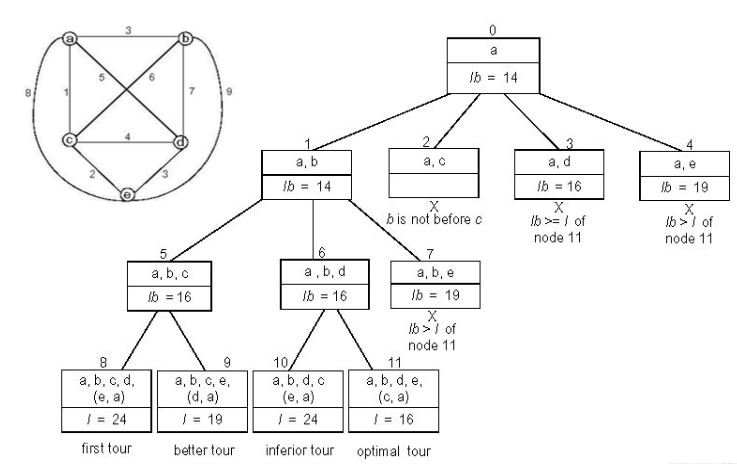
\includegraphics[width=4.5in] {TSP-Backtracking.png}
\end{figure}

}
 


%\frame{
%	\frametitle{Enumeration tree and backtracking}
%
%See an extra slide
%%\begin{figure}
%% 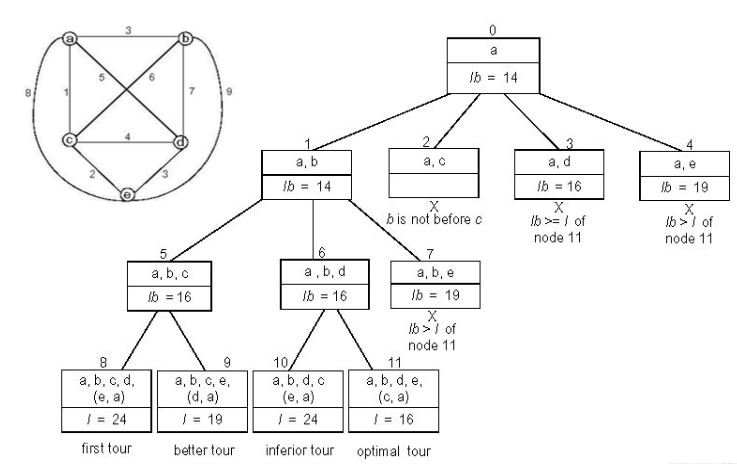
\includegraphics[width=4.5in] {TSP-Backtracking.png}
%%\end{figure}
%
%}


\frame{
	\frametitle{Backtracking}	
\begin{small}
\begin{algorithmic}[1]
\STATE{Start with the original problem $P_0$;}
\STATE{ Let $A = \{P_0\}$. Here $A$ denotes the active subproblems.}
\STATE{$bestsofar = \infty$};
\WHILE{ $A \neq NULL$ }
\STATE \textcolor{red}{\bf choose} a subproblem $P\in A$, and remove it from $A$;
\STATE \textcolor{red}{\bf expand} $P$ into smaller subproblems $P_1, P_2, ..., P_k$;
\FOR{$i=1$ to $k$}
\IF { \textcolor{red}{\bf $(P_i)$}  corresponds to a complete solution }
\STATE update $bestsofar$;
\ENDIF
\IF { \textcolor{red}{\bf lowerbound$(P_i) \leq bestsofar$}  }
\STATE insert $P_i$ into $A$;
\ENDIF
\ENDFOR
\ENDWHILE
\end{algorithmic}
\end{small}
}





\frame{
\begin{block}{}
{\bf Time complexity and space complexity}
\end{block}

}

\frame{
\frametitle{Time complexity and space complexity}

\begin{itemize}
	\item Time (space) complexity of an algorithm quantifies the time (space) taken by the algorithm. 
	\item Since the time costed by an algorithm grows with the size of the input, it is traditional to describe running time as a  function of the input size. 
	\begin{itemize}		
		\item \textcolor{blue}{\bf input size}: The best notation of input size depends on the problem being studied. 
			\begin{itemize}
				\item For the {\sc TSP} problem, the \textcolor{blue}{\tt number of cities in the input}. 
				\item For the {\sc Multiplication} problem, the \textcolor{blue}{\tt total number of bits} needed to represent the input number is the best measure. 
			\end{itemize}		  		
	\end{itemize}
\end{itemize}
} 

\frame{
\frametitle{Running time:  we are interested in its growth rate}
\begin{itemize}
	\item A straightforward way is to use the exact seconds that a program used. However, this measure highly depends on CPU, OS, compiler, etc. 
	\item Several  simplifications to ease  analysis of  Held-Karp  algorithm: 
	\begin{enumerate}
		\item  We simply use the number of primitive operations (rather than the exact seconds used) under the assumption that a primitive operation costs constant time. Thus the running time is $T(n) = a n^2 + b n + c $ for some constants $a, b, c$. 
		\item We consider only the leading term, i.e. $a n^2$, since the lower order terms are relatively insignificant for large $n$. 
		\item We also ignore the leading term's coefficient $a$ since the it is less significant than the growth rate. 
	\end{enumerate} 
	\item Thus, we have $T(n) = a n^2 + b n + c = O(n^2)$.  Here, the letter $O$ denotes \textcolor{blue}{order}.  
\end{itemize}
} 

\frame{
\frametitle{ \textcolor{red}{Big $O$}  notation } 

\begin{itemize}
	\item Recall that big $O$ notation is used to describe the \textcolor{blue}{\tt error term} in Taylor series, say: 
	
	\centering{$e^x = 1 + x + \frac{x^2}{2} + O(x^3)$ as $x\rightarrow 0 $ }
	
\end{itemize}

\begin{figure}
 \includegraphics[width=1.6in,angle=270] {L1-big-O.eps}
 \caption{Example: $f(x) = O(g(x))$ as there exists $c>0$ (e.g. $c=1$) and $x_0 = 5$ such that 
 $f(x) < c g(x)$ whenever $x>x_0$} 
\end{figure}

}

\frame{
\frametitle{ \textcolor{red}{Big $\Omega$} and  \textcolor{red}{Big $\Theta$}  notations } 

\begin{itemize}
\item 
In 1976 D.E. Knuth published a paper  to justify his use of the $\Omega$-symbol to describe a stronger property. Knuth wrote: "For all the applications I have seen so far in computer science, a stronger requirement [...] is much more appropriate". 

\item He defined

\begin{center} 
$f(x)=\Omega(g(x))\Leftrightarrow g(x)=O(f(x))$
\end{center}

with the comment: "Although I have changed Hardy and Littlewood's definition of $\Omega$, I feel justified in doing so because their definition is by no means in wide use, and because there are other ways to say what they want to say in the comparatively rare cases when their definition applies". 

\item Big $\Theta$ notation is used to describe ``$f(n)$ grows  asymptotically as fast as $g(n)$". 
\begin{center} 
$f(x)=\Theta(g(x))\Leftrightarrow g(x)=O(f(x)) $ and $f(x) = O(g(x))$. 
\end{center}

\end{itemize}
%However, the HardyÅ0â9Å0Å0Å0Ç9Littlewood definition had been used for at least 25 years.[13]
}

\frame{
	\frametitle{Worst case and average case} 
	
\begin{figure}
 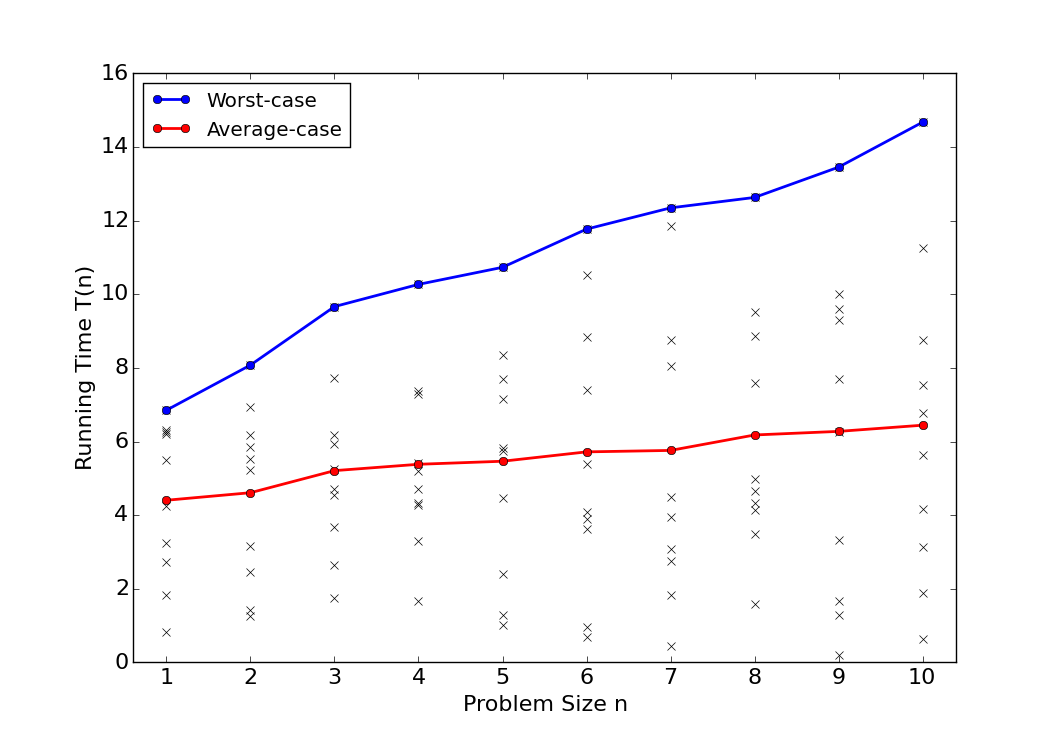
\includegraphics[width=3in] {WorstAverageCase.png}
\end{figure}
\begin{itemize}
	\item Worst-case: the case that takes the longest time; 
	\item Average-case: we need know the distribution of the instances; 
\end{itemize}
	
}



\end{document}
